\excercise{While i do stuff on repeat}

Ziel dieser Aufgabe ist es, die Syntax und die Funktion der While-Schleife genauer zu verstehen.
\begin{enumerate}[label=\alph*)]
    \item Zunächst betrachten wir ein paar einfache Programmausschnitte mit einer While-Schleife.
    Überlege dir, welche Ausgaben die jeweiligen Abschnitte machen:
    \begin{lstlisting}
System.out.println("Before");
boolean cond = true;
while(cond){
    System.out.println("While");
    cond = false;
    System.out.println("While");
}
System.out.println("After");

// --------------------------------------------------------

int count = 0;
while(count < 10){
    System.out.println(count);
    count++; //count = count + 1;
}
    \end{lstlisting}
    \item Instanziiere den Task und den Verifier. Dabei soll für jede Teilaufgabe nun ein SubTask angegeben werden, da zwischen
    den Teilaufgaben der Programmcode verändert werden soll:
    \begin{lstlisting}[breaklines=true]
SubTask subTask = SubTask.B;
Game myGame = new Game("Sheet2Task5", new Sheet2Task5(subTask), new Sheet2Task5Verifier(subTask));
myGame.run();
    \end{lstlisting}
    Starte den Task zwei Mal, was fällt dir auf?
    \item Nun sollen alle vor Neo liegenden Münzen aufgehoben werden. Bearbeite dazu die Methode \textit{subTaskC(Neo neo)} in der Klasse \textit{Sheet2Task5}.
    \item Finde eine Abfolge an Anweisungen für Neo, sodass in jedem Feld der mittleren Zeile genau eine Münze liegt. Implementiere deine Idee in der Methode
    \textit{subTaskD(Neo neo)}.
    \item Betrachte die folgende Abbildung des Spielfelds
    \begin{figure}[h!]
        \centering
        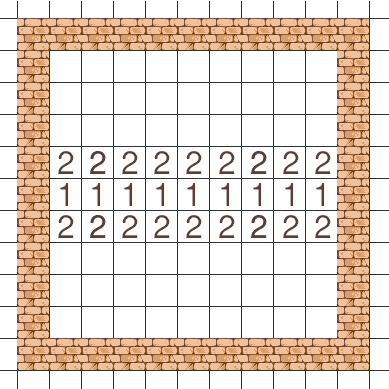
\includegraphics[height=5cm]{figures/ex05e.png}
    \end{figure}\newline
    Finde eine Abfolge an Anweisungen für Neo, sodass in jedem obigen markierten Feld die richtige Anzahl an Münzen vorkommt. Implementiere deine Idee
    in der Methode \textit{subTaskE(Neo neo)}.
    \newpage
    \item Implementiere nun das selbe Verhalten für die folgende Abbildung des Spielfelds.\\
    \begin{figure}[h!]
        \centering
        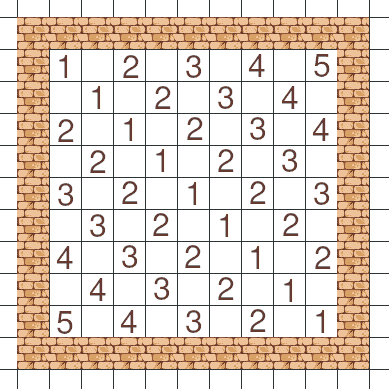
\includegraphics[height=5cm]{figures/ex05f1.png}
    \end{figure}\newline
    \item Wie müsste man den Programmcode in Teilaufgabe \textit{e)} und \textit{f)} abändern, so dass die Münzen nur ein Feldern liegen, an welchen 
    keine Wand angrenzt. Implementiere diese Änderung für Teilaufgabe \textit{e)}.\\
    \textit{Hinweis:} Es werden in den Reihen 2 und 6 zufällig Wände eingefügt, wodurch ihr die Implementierung etwas allgemeiner fassen müsst!
\end{enumerate}